\documentclass[Spanish,12pt,doublespace,german,letterpaper]{article}
\usepackage[T1]{fontenc}
\usepackage{pdfpages}
\usepackage[spanish]{babel}
\usepackage{latexsym}
\usepackage{enumerate}
\usepackage{amsmath}
\usepackage{amsbsy}
\usepackage{amssymb}
\usepackage{graphics}
\usepackage{graphicx}
\usepackage{color}
\usepackage{hyperref}
\DeclareGraphicsExtensions{.png,.pdf,.jpg,.mps,.eps}
\renewcommand{\baselinestretch}{1.5}  %Espaciamiento de lineas
\frenchspacing %control de espacios

% Título Portada
\centerline{\Large UNIVERSIDAD MAYOR DE SAN ANDRÉS}
\centerline{FACULTAD DE CIENCIAS PURAS Y NATURALES}
\centerline{POSTGRADO AUTOFINANCIADO
EN MATEMÁTICA} 
\centerline{Módulo II: Matrices} 
\vspace{12em}
\centerline{\huge RAIZ DE  MATRICES  MEDIANTE }\vspace{1em}
\centerline{\huge SCHUR APLICADO A VISION ARTIFICAL}\vspace{1em}
 \centerline{\huge  REJILLAS DE FRECUENCIA}\vspace{1em}
 \centerline{\huge (EN T.F. FOURIER ) }
\vspace{10em} \centerline{\Large EDGAR DANIEL TÁRRAGA
TORREZ}\vspace{4em}
 \centerline{\Large Tarija, julio 2023}\vspace{5em}
 \pagebreak
\begin{document}
\tableofcontents
\pagenumbering{arabic}
\newpage

En el  procesamiento de imagenes la importancia de la Transformada de Fourier  se desarrollo con  métodos numéricos que permiten su uso en contexto computacional. 
La TF discreta permite encontrar una función espectral discreta (es decir, para una secuencia finita de N frecuencias) a partir de una señal discreta de N valores:


La misma formulación de la transformada discreta se aplica a señales 2D (imágenes), aprovechando otra propiedad fundamental de la TF, denominada separabilidad (la TF de una función 2D que puede ponerse como producto de dos funciones 1D, es el producto de cada una de las TF de dichas funciones).
De esa forma surge la TF discreta para funciones 2D f(nx, ny), donde Fh y Fv representan frecuencias horizontales y verticales, respectivamente (en este caso se trata de frecuencias geométricas):

 

Una forma de representar la TF de una imagen es con otra imagen de igual resolución. 
En si Fh y Fv representa una matriz nueva del espectro de frecuencias el cual se  utiliza  alguna forma de pseudocolor para representar la energía a cada una de las frecuencias el cual estas nos dan los paramteros de ruidos,nitidez,etc sobre la imagen.
Dicho esto el tratamiento de esta repesentacion grafica de forurier  tiene un campo grande donde existen numerosas propuestas aplicadas para mejorar imagenes. 



\subsection{Planteamiento del problema}
La TF de las imagenes con una interferencia aditiva se puede observar que  algunos  puntos simétricos donde esa interferencia está localizada en el espectro. 

\begin{figure}[h]
\begin{center}
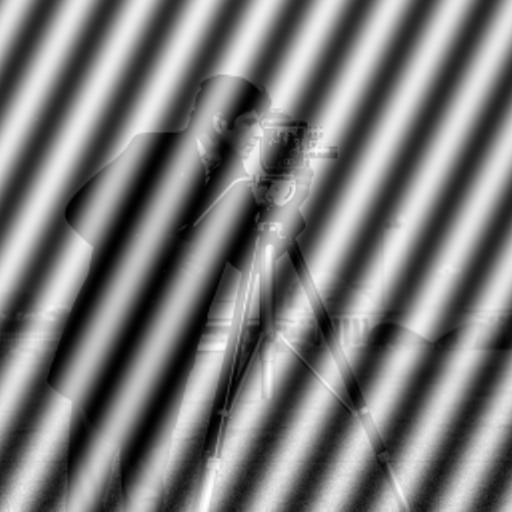
\includegraphics[scale=0.4]{tp4.jpg}
\caption{Imagen con frecuencias aditivas}
\label{default}
\end{center}
\end{figure}
Si editamos el espectro y eliminamos la energía a esas frecuencias se puede restaurar la imagen original.
\begin{figure}[h]
\begin{center}
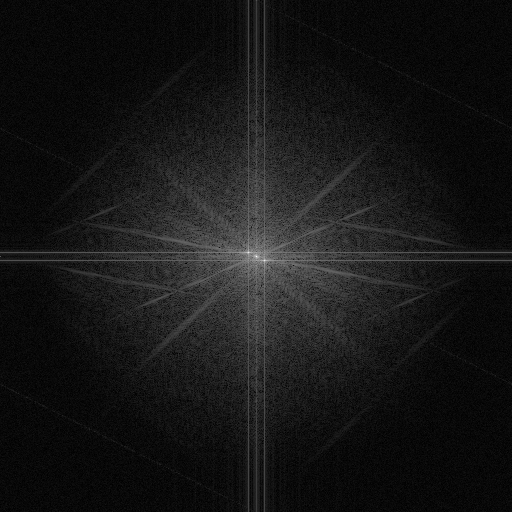
\includegraphics[scale=0.4]{log_center_mag.png}
\caption{Imagen logariotmica sin tratar}
\label{Imagen logariotmica sin tratar}
\end{center}
\end{figure}
En resumen una de las técnicas iníciales es hacer la captura de la imagen de la T.F. y determinar un aplicativo manual que elimine los puntos blancos concentrados de energia y esto dara un efecto, modificatorio a  la TF y se realizia  la transformada inversa con el espectro manipulado( Imagen corregida ), y se logra corregir casi por completo el defecto en la imagen original.

\begin{figure}[h]
\begin{center}
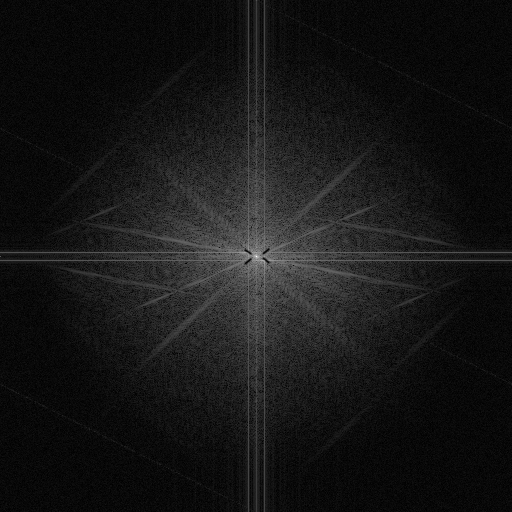
\includegraphics[scale=0.4]{log_center_mag2.png}
\caption{Imagen logariotmica con tratamiento}
\label{Imagen logariotmica con tratamiento}
\end{center}
\end{figure}
\subsection{Justificacion}
Mediante aplicativos de Python se pretende   encontrar  la matriz de modulo y angulo de la descomposion de Fourier en 2D , el cual con estas matrices se buscara en filas y columnas los puntos altos de concentracion de frecuencias y asi recuadrar rejillas 2x2 para sus tratamiento  
El tratamiento que se pretende usar las tecnicas de descomposiion de matrices  mediante schur (factorizacion)  estudiadas en el modulo II de matrices y asi mismo calcular la raiz matricial de esta rejilla y reemplazar en la matriz principal, este proceso de tratamiento de rejillas de 2x2 se hara con dos iteracciones.
\subsection{Objetivo General.}
El presente proyecto  tiene por objetivo desarrollar un aplicativo/formulacion  en python para hallar la raiz cuadrada  de una matrizy mediante schur ,asi mismo este tratamiento de raiz cuadrada se aplicara  a rejillas 2x2 en puntos maximos de la mtariz principal de frecuencias  el cual reemplazara en las rejillas/matrices 2x2, y con  este proceso de tratamiento de rejillas/matrices de 2x2 llegar a  dos iteracciones. para ver su mejoramiento
\subsection{Objetivos Especificos.}
Entre los objetivos especificos que se pretende alcanzar son:
\begin{itemize}
  \item Desarrollo de ecuaciones para calcular autovalores y autovectores en python para matrices 2x2 
  \item Desarrollo de ecuaciones para la descomposion de Grand Schmit.
  \item Desarrollo de de ecuaciones   para el calculo de raiz cuadra mediante schur
  \item Desarrollo de aplicativos de jupiter notebook para codificacion en  python de las ecuaciones a usar en este proyecto
  \item Desarrollo de aplicativos en python para visualizar el espectro de Foruier.
 \end{itemize}
 
\section{Fundamentos Teoricos}
\subsection{Polinomio caracteristiv}
Sea f : V → V una aplicaci ́on lineal con matriz asociada A en una cierta base.


Se sabe que 
$$f(x) = Ax$$ 
Si x es un autovector asociado a un autovalor λ, entonces
$$f(x) = λx ⇒ Ax = λx ⇒ (A − λI)x = 0$$
Denotando por $A = (a_{ij})$ y $x = (x_1,...,x_n)$, podemos escribir estas ecuaciones expl ́ıcitamente como
\begin{equation}
\begin{matrix}
 (a_{11}-\lambda)x_1    & + & a_{12}x_2          & +\cdots & a_{1n}x_n       & =  & 0\\
  a_{21}x_1             & + & (a_{22}-\lambda)x_2  & +\cdots & a_{2n}x_n       & =  & 0\\
 \vdots & \vdots        &        & \vdots & \vdots \\
  a_{n1}x_1             & + & a_{n2}x_2   & \cdots & (a_{nn}-\lambda)x_n &  =  & 0
\end{matrix}
\end{equation}
Obteniendo un sistema homogeneo que debe satisfacer cada uno de los auto-vectores asociados al autovalor λ.

Ası pues, para que existan autovectores, este sistema debe tener solucio ́n distinta de la trivial, o equivalentemente, la matriz del sistema debe tener rango menor que n. 
Esto es,

\begin{equation}
\begin{vmatrix}
  a_{11}-\lambda    & + & a_{12}          & +\cdots & a_{1n}       \\
  a_{21}            & + & a_{22}-\lambda  & +\cdots & a_{2n}       \\
 \vdots & \vdots        &        & \vdots & \vdots \\
  a_{n1}             & + & a_{n2}x_2   & \cdots & a_{nn}-\lambda 
\end{vmatrix}
\end{equation}

$$|A -\lambda I_n|=0$$
\section{Algortimo Raiz mediante Schur}
Se aplica un algprtimo en python para el calculo de la raiz cuadrada de matrices 2x2 , qeu seran las rejillas encontradas en la matriz de magnitud. 
\includepdf[pages=-]{RaizMatriz}
\section{Desarrollo }
El objetivo, de extraer las graficas de la transformada de fourier de la figura con frecuencias aditivas, una vez extraidas se forma una matriz denominada 
\begin{equation}
\begin{vmatrix}
fft2_center_mag:Matriz dela magnitud de Fourier \\
fft2_center_ang :Matriz del angulo de Fourier 
\end{vmatrix}
\end{equation}
Se trabaja en la matriz de magnitud con el siguiente algoritmo propuesto:
\begin{figure}[h]
\begin{center}
\includegraphics[scale=0.35]{Algoritmo.jpeg}
\caption{Algotimo propuesto}
\label{Algoritmo Propuesto}
\end{center}
\end{figure}
Se busca en la matriz de magnitud el valor maximo , el cual se ubica como a11 de una matriz 2x2, el cual mediante descomposicion de schur, se efectua 
el calculo de la matriz raiz y luego se reemplaza en la rejilla de 2x2 , el  cual se vuelve a invertir y se encuentra la imgane tratada.
\includepdf[pages=-]{Fourier_RaizMatriz}
\section{Conclusiones}
Se verifica que en matrices de 2x2 , es muy optimo el tratamiento con tres iteracciones .
El proyecto esta alojado en la siguiente direccion github:


\url{https://github.com/tarraga888/Maestria-UMSA-mod2/tree/0c2ec8fb767b97d45402391852531444fe3f0041/Proyecto_EDTT}


Se efetuara a futuro el tratameinto para que el valor maximo encontrado a tratar forme parte de una matriz 3xs3  el cual el maximo seria a22.

Con las iteracciones se comprueba que la ayuda de matrices efectua un tratamiento similar al de convoluciones.
\end{document}
